\documentclass[aspectratio=43,t]{beamer}
%\documentclass[aspectratio=43,t,handout]{beamer}

\usepackage[ansinew]{inputenc}
\usepackage[T1]{fontenc}
\usepackage[english]{babel}
\usepackage{amsmath,amssymb}
\usepackage{graphicx}
\usepackage{listings}
\usepackage{verbatim}
\usepackage[backend=biber,sorting=ydnt,doi=true]{biblatex}
\usepackage{adjustbox}
\usepackage{subfigure}


\usepackage{wrapfig}
\usepackage{chngcntr}
\setbeamertemplate{caption}[numbered]
\usepackage{listings}

\usepackage{amssymb}% http://ctan.org/pkg/amssymb
\usepackage{pifont}% http://ctan.org/pkg/pifont
\newcommand{\cmark}{\ding{51}}%
\newcommand{\xmark}{\ding{55}}%

% Themes:
%  - fau:          Default FAU theme
%  - fau-tf:       TechFak FAU theme
%  - fau-tf-hscd:  Co-Design FAU theme
%
% Options:
%  - seal:         FAU seal on title page (default)
	%  - logo:         Beamer logo on all pages
	%  - image:        Cover image on title page
	%  - plain:        Plain title page
	%  - longtitle:    Title page layout for long title
	%  - dark:         Dark version of theme
	\usetheme[seal, longtitle]{fau-tf}
	%\setbeamercovered{transparent}


	\lstset{%
		language=C++,
			tabsize=2,
			basicstyle=\tt\scriptsize,
			keywordstyle=\color{blue},
			commentstyle=\color{green!50!black},
			stringstyle=\color{black},
			% stringstyle=\color{red},
			numbers=left,
			numbersep=0.5em,
			numberstyle=\tt\tiny
	}


\defbibheading{bibliography}{}
\addbibresource[label=primary]{references.bib}
\nocite{*}


% Title, authors, and date
\title[SmartBierdeggl]{SmartBierdeggl}
\subtitle{DIY: Abschlussvortrag}
\author[Achim Herrmann/Daeubler]{Achim Herrmann/Daeubler}
\institute[Rechnernetze und Kommunikationssysteme]{Rechnernetze und Kommunikationssysteme, Friedrich-Alexander-Universit�t Erlangen-N�rnberg}
\date{\today}

\begin{document}
% Title
\frame[plain,c,noframenumbering]{\titlepage}

\begin{frame}{Idee}
                \begin{center}
        \begin{adjustbox}{max width=.8\textwidth, max height=.8\textheight}
                        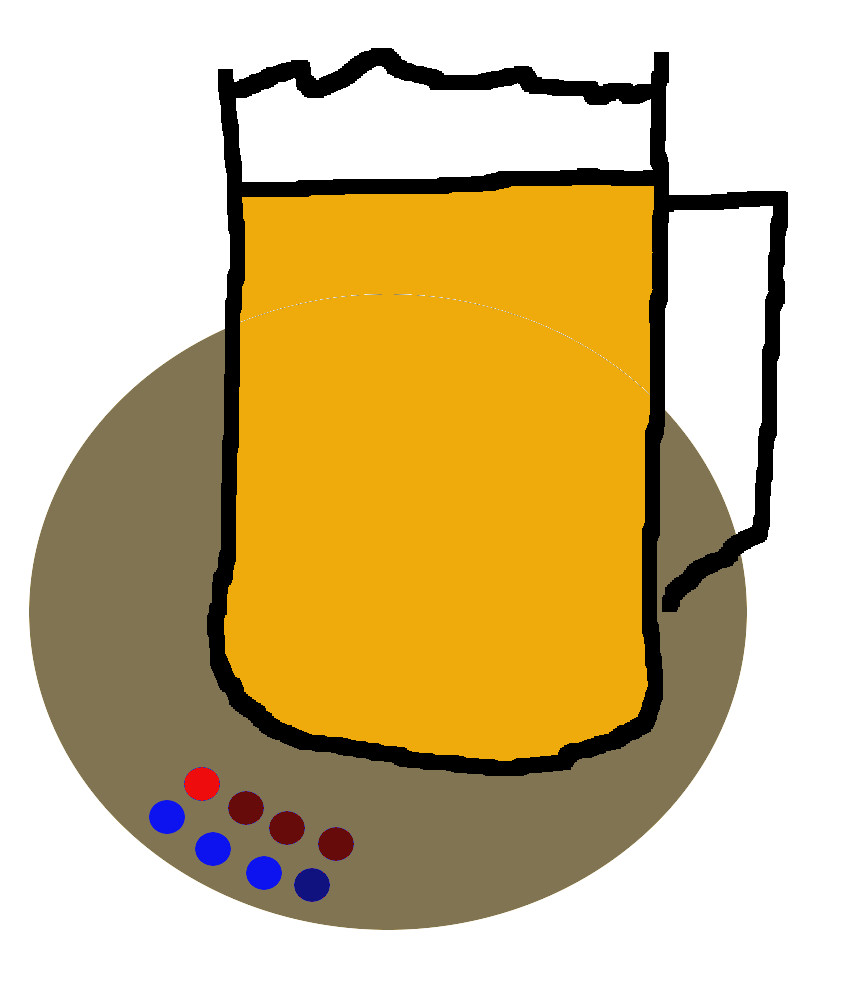
\includegraphics[]{images/idee}
%        \end{adjustbox}
%        \begin{adjustbox}{max width=.4\textwidth, max height=.4\textheight}
                        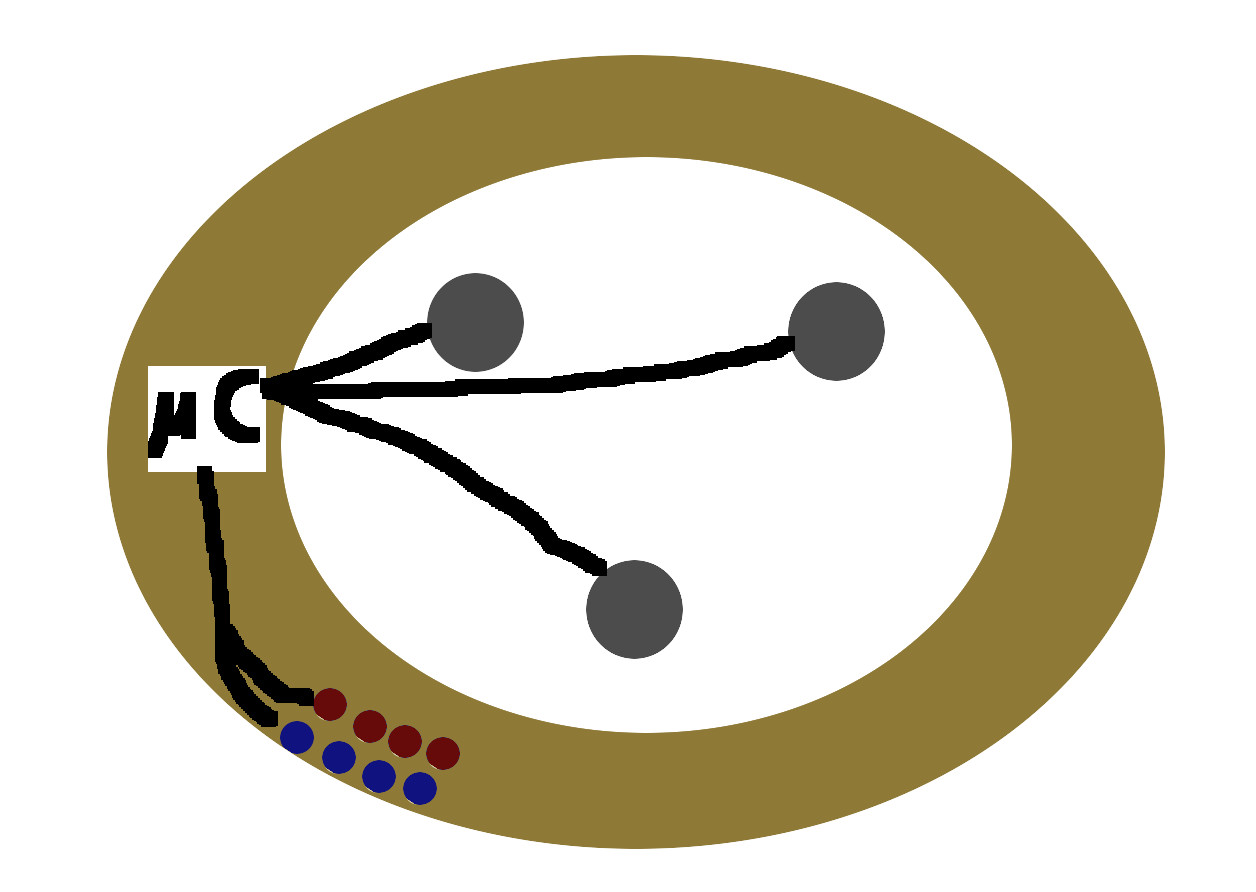
\includegraphics[]{images/aufbau}
        \end{adjustbox}
                \end{center}
\end{frame}
\begin{frame}{Aktueller Stand}
                \begin{center}
        \begin{adjustbox}{max width=.8\textwidth, max height=.8\textheight}
                        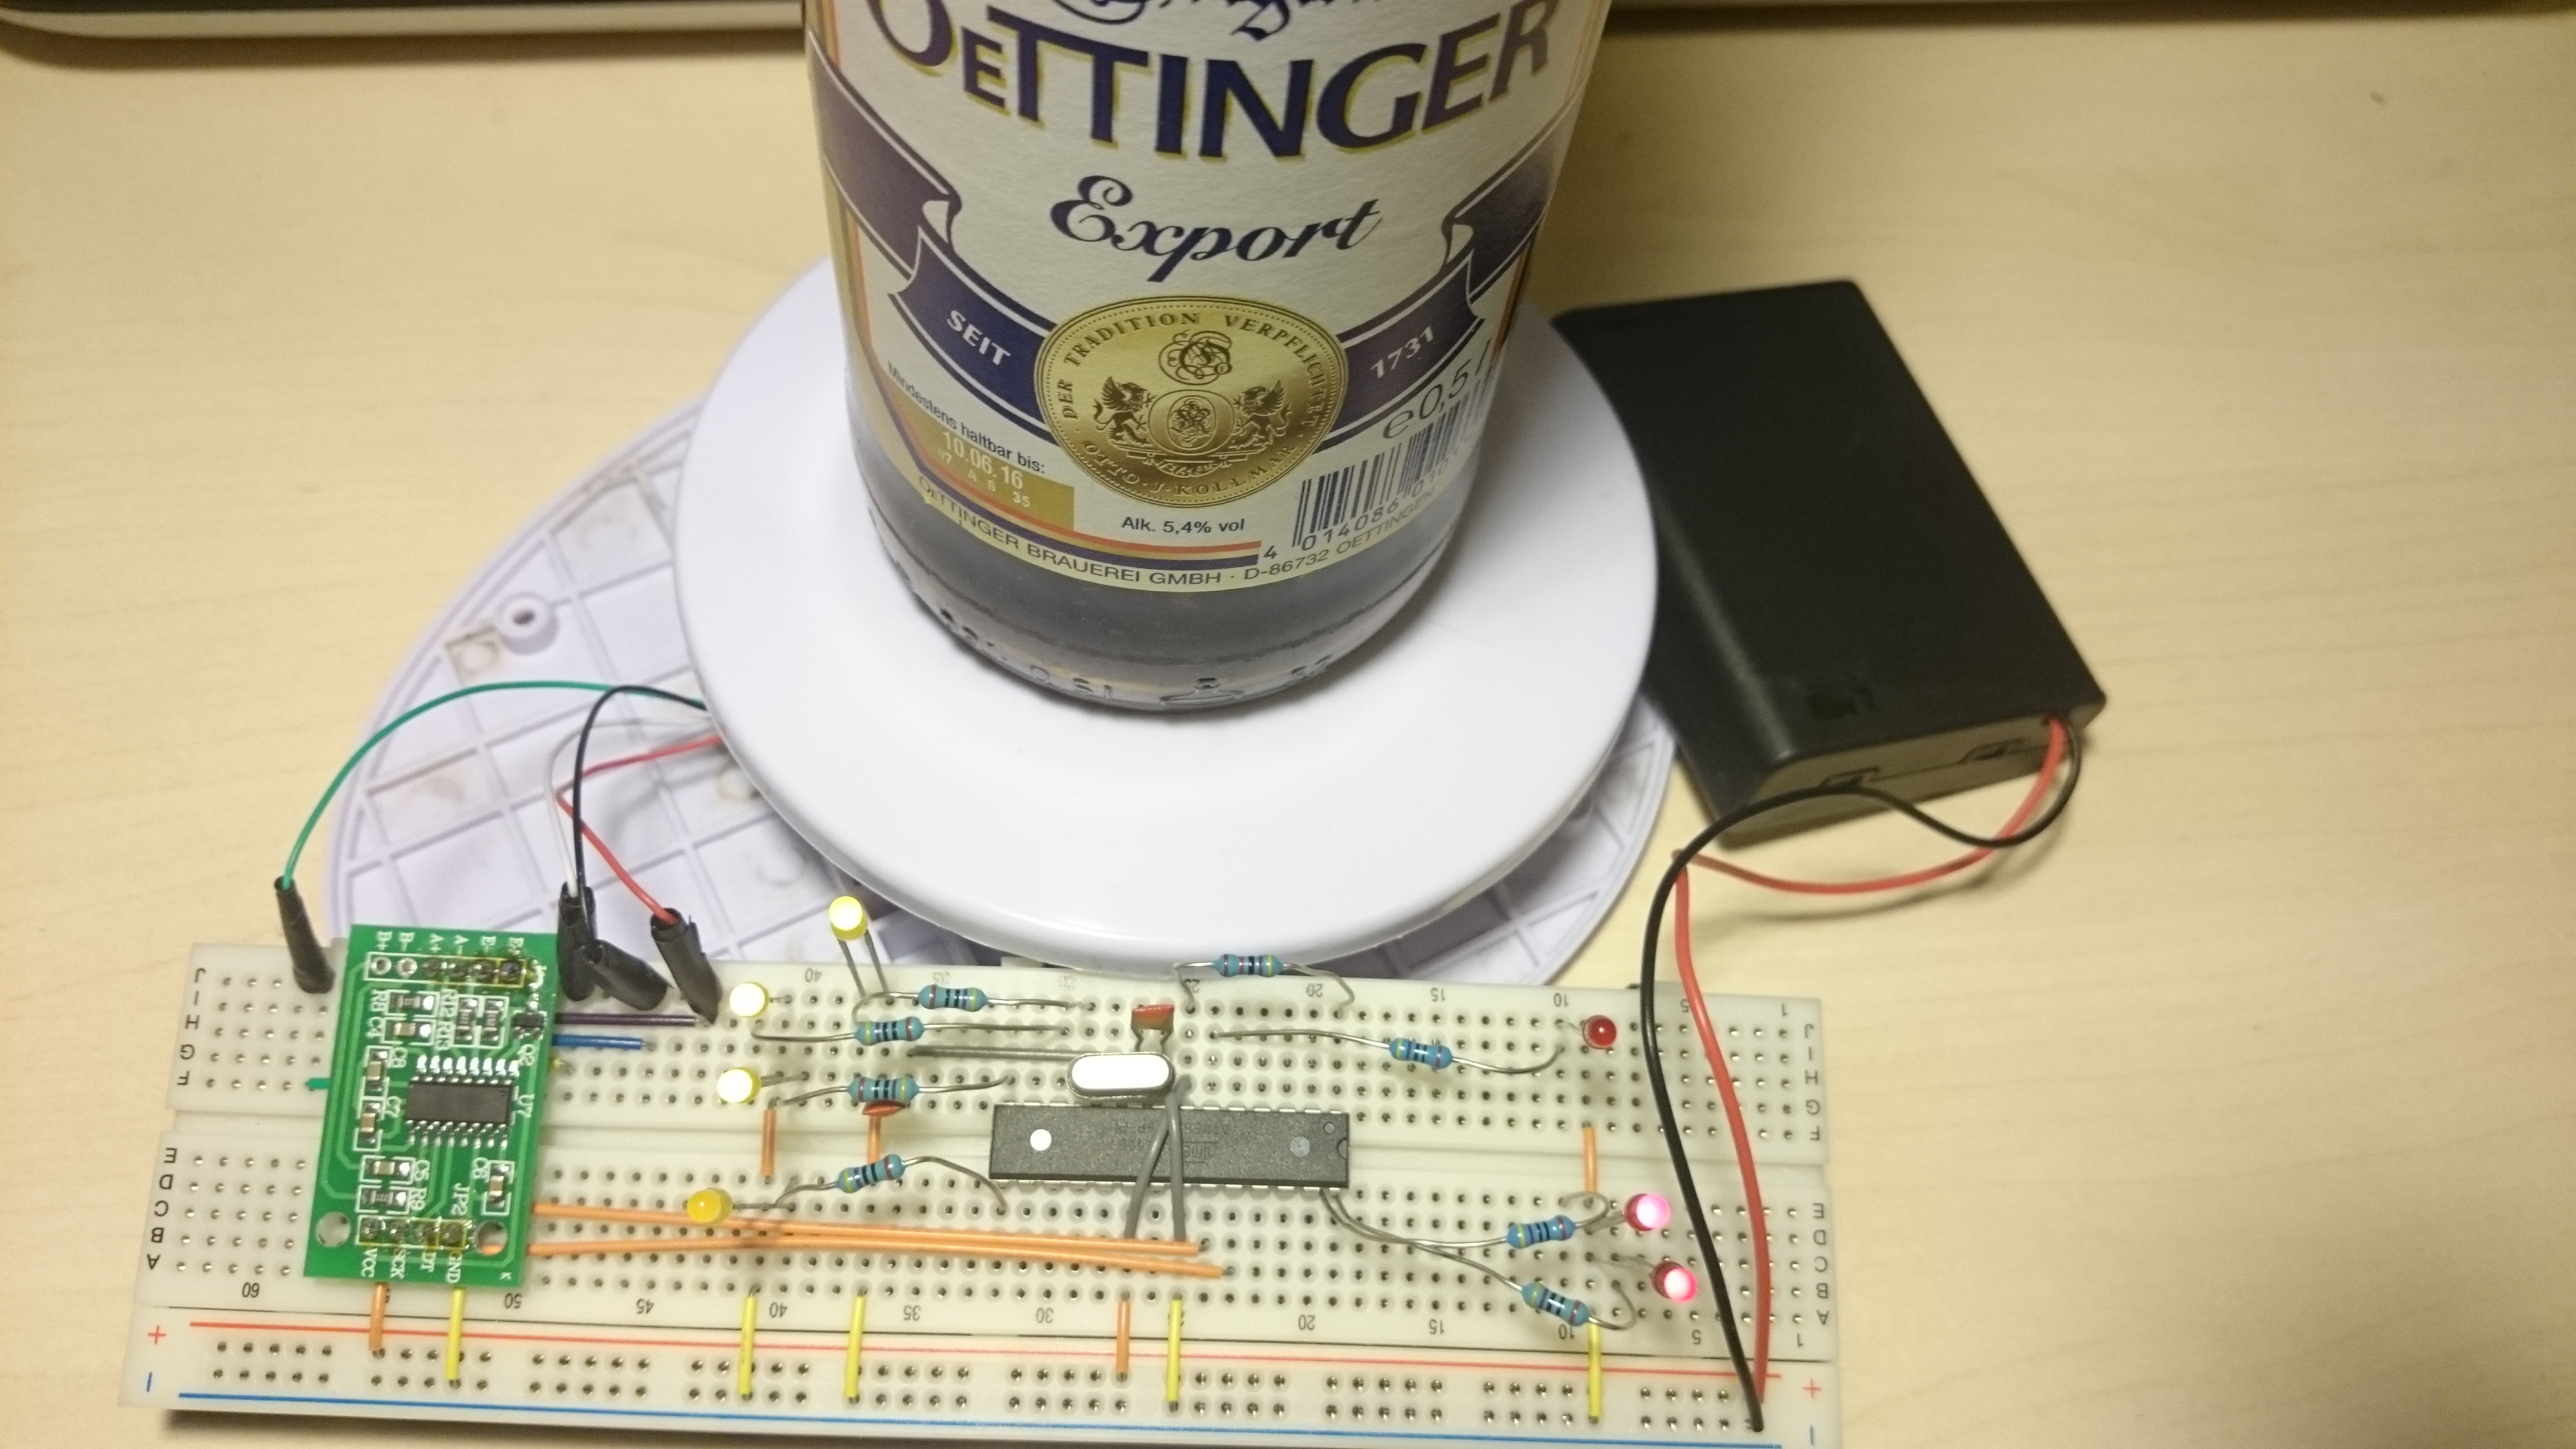
\includegraphics[trim=0 0 500 0,clip]{images/prototype} %l b r u
        \end{adjustbox}
                \end{center}

\end{frame}
\begin{frame}{Wiegeeinheit}

                
        \begin{itemize}
        \item W�gezelle mit Dehnmessstreifen (Wheatstone'sche Br�ckenschaltung)
        	\begin{figure}
        	        \begin{adjustbox}{height=.3\textheight}
                        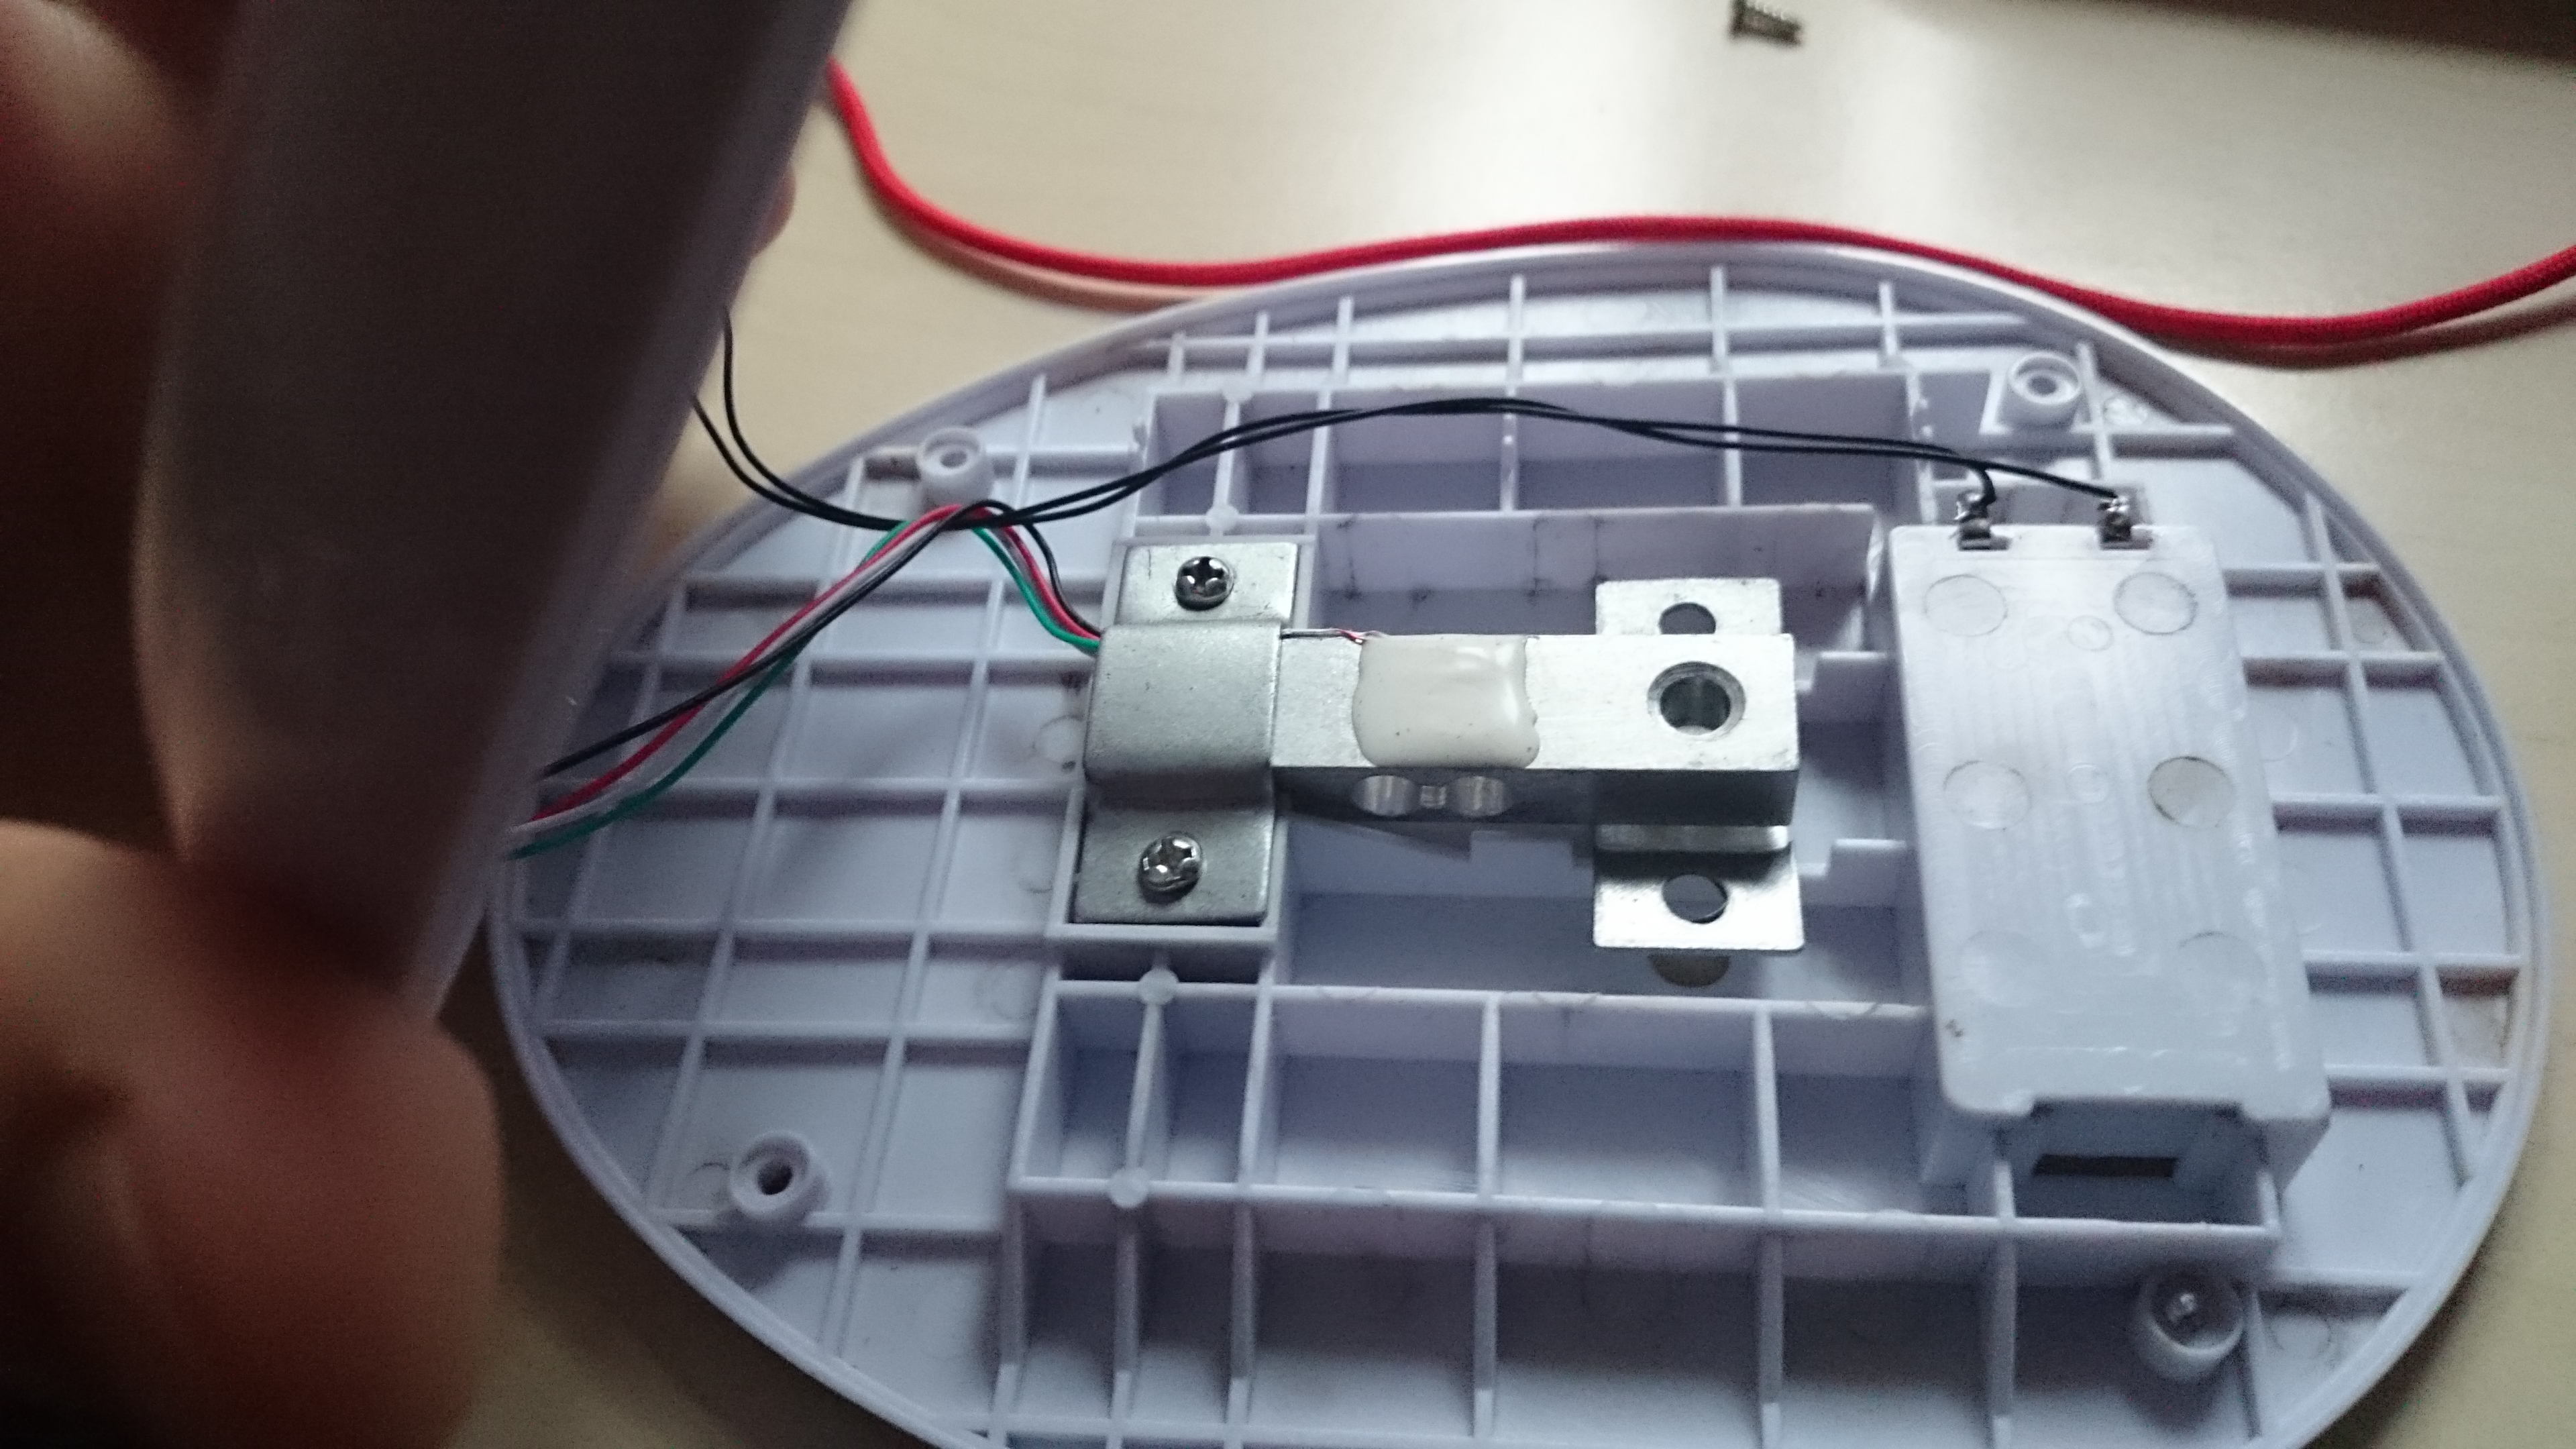
\includegraphics[trim=1250 500 650  500,clip]{images/loadcell} 
        \end{adjustbox}
        	\end{figure}
        \item HX711: 24 bit ADC
        \begin{figure}
        	        \begin{adjustbox}{height=.3\textheight}
                        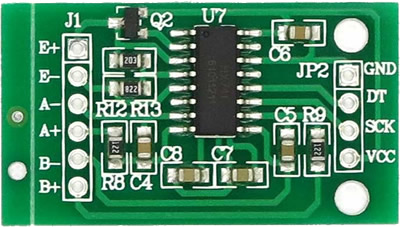
\includegraphics[]{images/hx711}
        \end{adjustbox}
        \end{figure}
        \end{itemize}

\end{frame}

\begin{frame}{Schaltplan}
  \begin{adjustbox}{height=.9\textheight}
	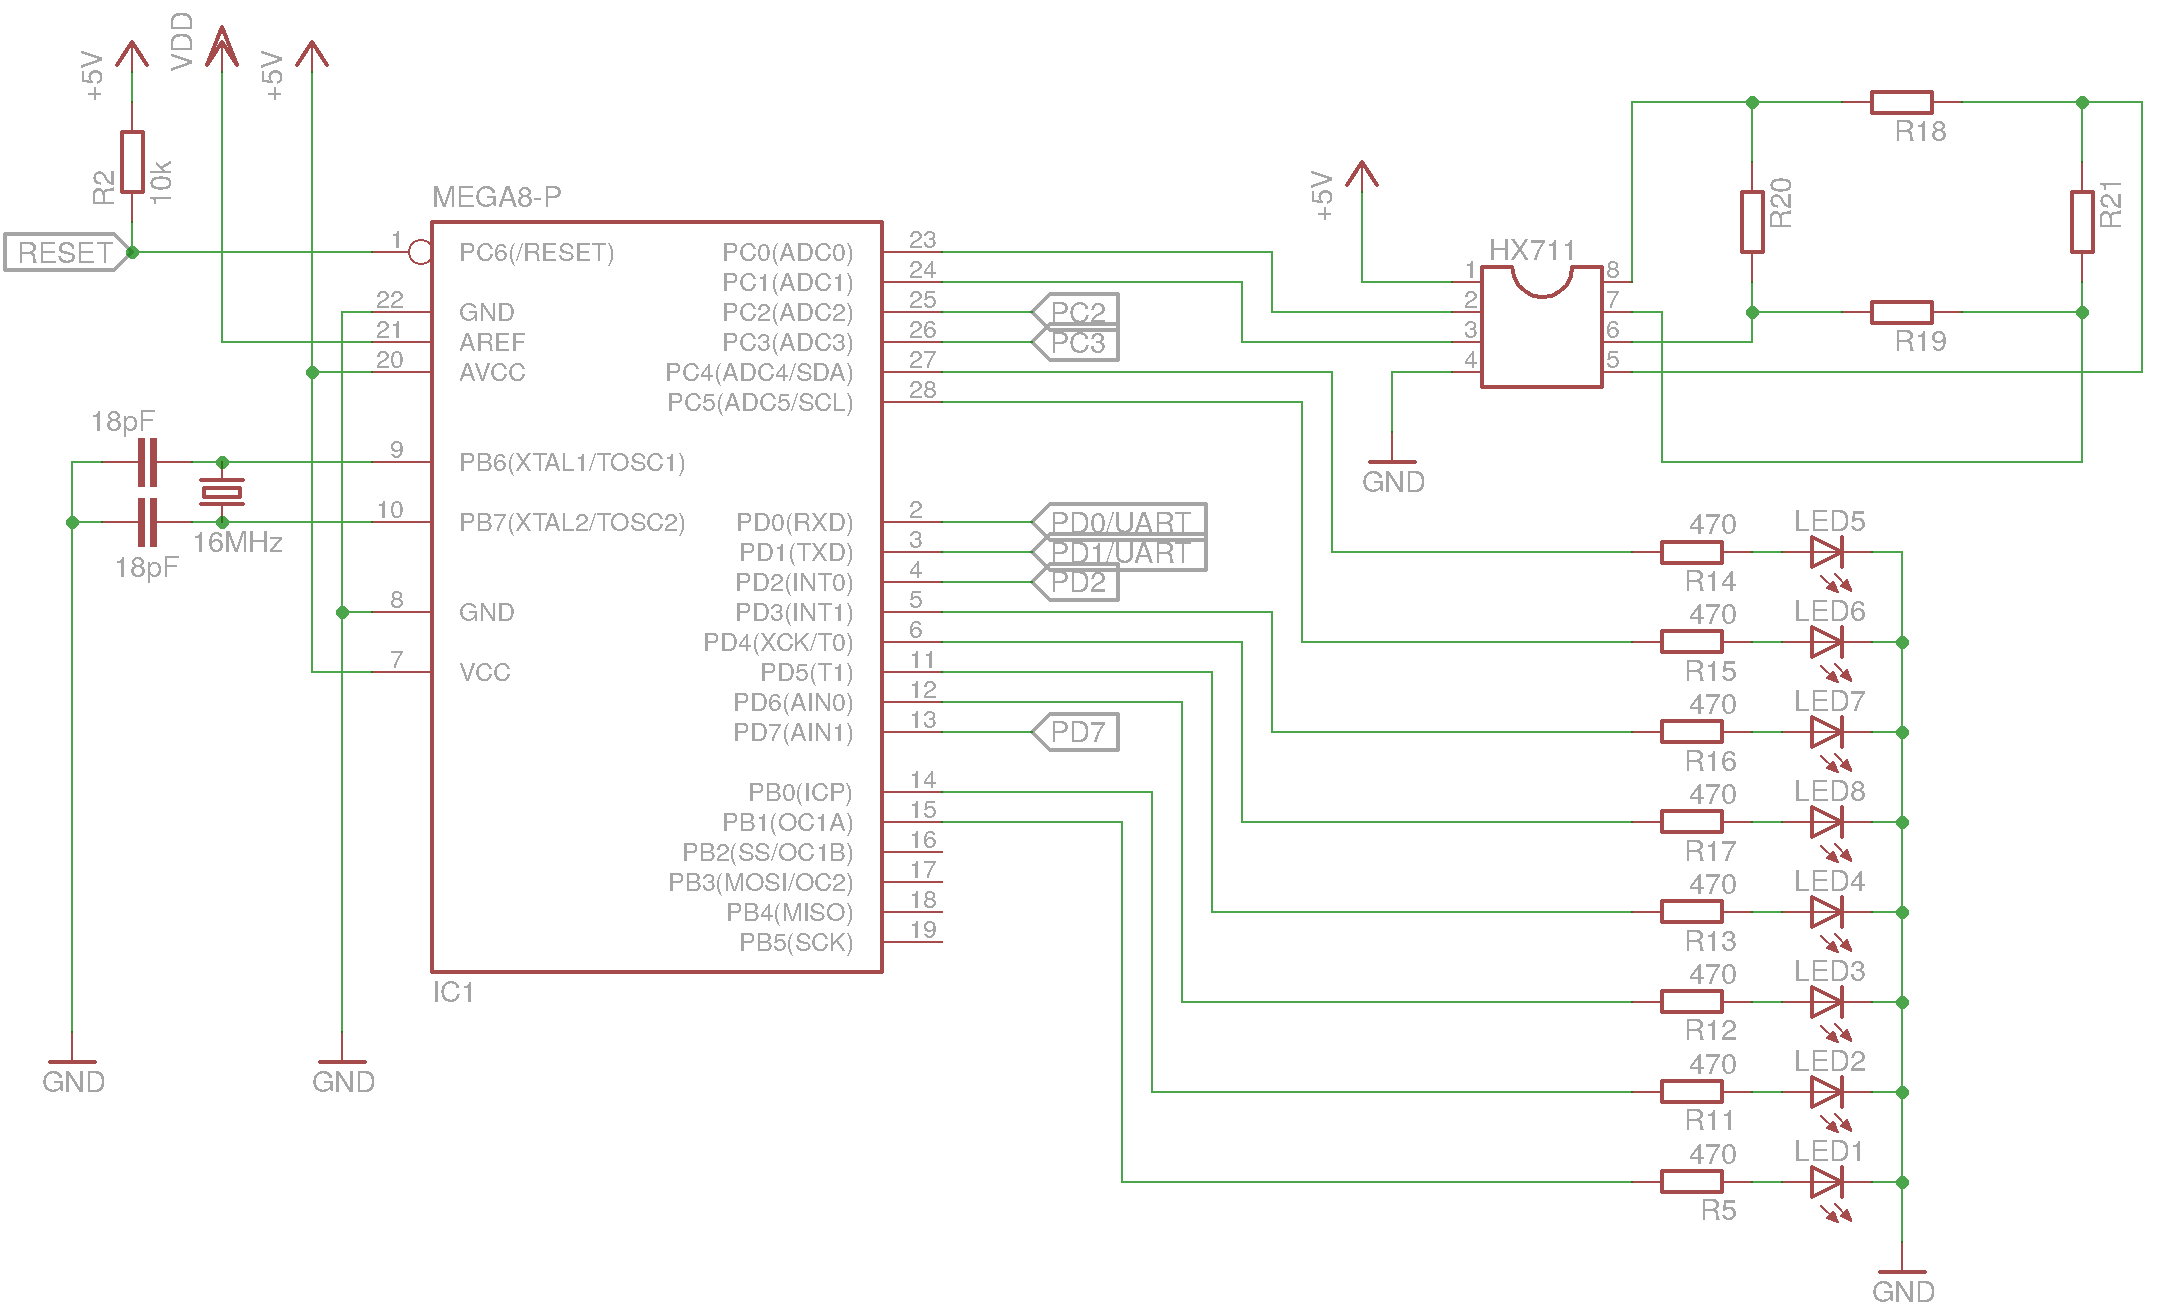
\includegraphics[]{images/board_complete}
   \end{adjustbox}
\end{frame}

\begin{frame}
\lstinputlisting[]{code/main.c}
\end{frame}
\begin{frame}
\lstinputlisting[]{code/hx711.c}
\end{frame}

{ % Questions?
	\setbeamertemplate{footline}{}
	\begin{frame}[c,noframenumbering]
		\begin{center}
	Danke f�r ihre Aufmerksamkeit.\\
	{\bf Noch Fragen?}
	\end{center}
	\end{frame}
}
\end{document}

